\documentclass[12pt, a4paper, onecolumn, oneside, final]{report}

\usepackage{telkomskripsi}

% Judul laporan. 
\var{\judul}{PERANCANGAN DAN SIMULASI\\
	PERLINDUNGAN PROPERTI INTELEKTUAL\\
	MENGGUNAKAN ALGORITME FILTER DIGITAL}

% Tulis kembali judul laporan, kali ini akan diubah menjadi huruf kapital
\Var{\Judul}{PERANCANGAN DAN SIMULASI
	PERLINDUNGAN PROPERTI INTELEKTUAL
	MENGGUNAKAN ALGORITME \textit{OBFUSCATION} FILTER DIGITAL}

\Var{\Judulen}{DESIGN AND SIMULATION OF INTELECTUAL PROPERTIES PROTECTION USING DIGITAL FILTER ALGORITHM}
% Tulis kembali judul laporan namun dengan bahasa Ingris
\var{\judulInggris}{Unknown Title for Final Report/Thesis/Disertation}

% Tipe laporan, dapat berisi Skripsi, Tugas Akhir, Thesis, atau Disertasi
\var{\type}{PROPOSAL TUGAS AKHIR}

% Tulis kembali tipe laporan, kali ini akan diubah menjadi huruf kapital
\Var{\Type}{PROPOSAL TUGAS AKHIR}

% Tulis nama penulis 
\var{\penulis}{Hanjara Cahya Adhyatma}

% Tulis kembali nama penulis, kali ini akan diubah menjadi huruf kapital
\Var{\Penulis}{Hanjara Cahya Adhyatma}

% Tulis NPM penulis
\var{\npm}{1104131113}
\var{\nim}{1104131113}
\var{\alamat}{Komplek BPI Blok E1 No. 16 RT 05 RW 06 Kabupaten Pandeglang, Banten}
\var{\email}{adhyatma.han@gmail.com}
\var{\tlp}{+6285201740588}
% Tuliskan Fakultas dimana penulis berada
\Var{\Fakultas}{Teknik Elektro}
\var{\fakultas}{Tekniks Elektos}

% Tuliskan Program Studi yang diambil penulis
\Var{\Program}{S1 Sistem Komputer}
\var{\program}{S1 Sistems Komputers}

% Tuliskan tahun publikasi laporan
\Var{\bulanTahun}{September 2017}
\Var{\Tahun}{2017}
% Tuliskan gelar yang akan diperoleh dengan menyerahkan laporan ini
\var{\gelar}{Sarjana Teknik}

% Tuliskan tanggal pengesahan laporan, waktu dimana laporan diserahkan ke 
% penguji/sekretariat
\var{\tanggalPengesahan}{XX September 2017} 

% Tuliskan tanggal keputusan sidang dikeluarkan dan penulis dinyatakan 
% lulus/tidak lulus
\var{\tanggalLulus}{XX September 2017}

\var{\pembimbing}{Prof. XXXX}
\var{\pembimbingSatu}{Surya Michrandi Nasution, S.T., M.T.}
\var{\pembimbingDua}{Fairuz Azmi, S.T., M.T.}

\var{\saya}{Hanjara Cahya Adhyatma}

\Var{\kataPengantar}{Kata Pengantar}
\Var{\babSatu}{Pendahuluan}
\Var{\babDua}{Tinjauan Pustaka}
\Var{\babTiga}{Desain dan Simulasi}
\Var{\babEmpat}{Pengujian dan Analisis}
\Var{\kesimpulan}{Kesimpulan dan Saran}


\hyphenation{
    % alphabhet A
    a-na-li-sa a-tur 
    a-pli-ka-si 
    % alphabhet B
    ba-ngun-an 
    be-be-ra-pa 
    ber-ge-rak
    ber-ke-lan-jut-an 
    ber-pe-nga-ruh
    ber-kurang 
    % alphabhet C
    ca-ri
    % alphabhet D
    di-sim-pan di-pim-pin de-ngan da-e-rah di-ba-ngun da-pat di-nya-ta-kan 
    di-sim-bol-kan di-pi-lih di-li-hat de-fi-ni-si
    % alphabhet E
    e-ner-gi eks-klu-sif
    % alphabhet F
    fa-si-li-tas
    % alphabhet G
    ga-bung-an ge-rak
    % alphabhet H
    ha-lang-an
    % alphabhet I
    % alphabhet J
    % alphabhet K
    ke-hi-lang-an
    ku-ning 
    kua-li-tas 
    ka-me-ra 
    ke-mung-kin-an 
    ke-se-pa-ham-an
    ke-rugian
    % alphabhet L
    ling-kung-an
    % alphabhet M
    me-neng-ah
    meng-a-tas-i me-mung-kin-kan me-nge-na-i me-ngi-rim-kan 
    meng-u-bah meng-a-dap-ta-si me-nya-ta-kan mo-di-fi-ka-si
    meng-a-tur
    % alphabhet N
    nya-ta non-eks-klu-sif
    % alphabhet O
    % alphabhet P
    pe-neliti-an
	pe-nye-rap-an 
	pe-ngon-trol
    pe-mo-del-an
    pe-ran  pe-ran-an-nya
    pem-ba-ngun-an pre-si-den pe-me-rin-tah prio-ri-tas peng-am-bil-an 
    peng-ga-bung-an pe-nga-was-an pe-ngem-bang-an 
    pe-nga-ruh pa-ra-lel-is-me per-hi-tung-an per-ma-sa-lah-an 
    pen-ca-ri-an peng-struk-tur-an
    % alphabhet Q
    % alphabhet R
    ran-cang-an
    % alphabhet S
    si-mu-la-si sa-ngat
    % alphabhet T
    te-ngah
    ter-da-pat
    % alphabhet U
    % alphabhet V
    % alphabhet W
    % alphabhet X
    % alphabhet Y
    % alphabhet Z
    % special
}

\var{\license}{\f{Creative Common License 1.0 Generic}}
\var{\bslash}{$\setminus$}

\begin{document}
% Sampul Laporan
\begin{titlepage}
    \begin{center}    
        \begin{figure}
            \begin{center}
                
\includegraphics[width=2.5cm]{pics/makara.png}
            \end{center}
        \end{figure}    
        \vspace*{0cm}
        \bo{
        	UNIVERSITAS TELKOM\\
        }
        
        \vspace*{1.0cm}
        % judul thesis harus dalam 14pt Times New Roman
        \bo{\Judul} \\[1.0cm]

        \vspace*{2.5 cm}    
        % harus dalam 14pt Times New Roman
        \bo{\Type}

        \vspace*{3 cm}       
        % penulis dan npm
        \bo{\Penulis} \\
        \bo{\npm} \\

        \vspace*{5.0cm}

        % informasi mengenai fakultas dan program studi
        \bo{
        	FAKULTAS \Fakultas\\
        	PROGRAM STUDI \Program \\
        	BANDUNG \\
        	\bulanTahun
        }
    \end{center}
\end{titlepage}


% Gunakan penomeran romawi
\pagenumbering{roman}

% load halaman judul dalam
\addChapter{HALAMAN JUDUL}
\begin{titlepage}
    \begin{center}
        \vspace*{1.0cm}
        % judul thesis harus dalam 14pt Times New Roman
        \bo{\Judul} \\[1.0cm]
        %\bo{\f{\Judulen}} \\[1.0cm]
        % harus dalam 14pt Times New Roman
        \bo{\Type} \\
        Kelompok Kompetensi : Arsitektur Komputer \\[1.0cm]
        % keterangan prasyarat
        %\bo{Disusun sebagai syarat untuk memperoleh gelar \gelar \\ pada Program Studi \program\\ Universitas Telkom}\\[1.0cm]
		\bo{oleh}\\[1.0cm]
        % penulis dan npm
        \bo{\Penulis} \\
        \bo{\npm} \\

		\begin{figure}
			\begin{center}
				
\includegraphics[width=3.5cm]{pics/telu.png}
			\end{center}
		\end{figure}    

        % informasi mengenai fakultas dan program studi
        \bo{FAKULTAS \Fakultas\\
        	UNIVERSITAS TELKOM\\
        	BANDUNG \\
        	\Tahun}
    \end{center}
\end{titlepage}

% setelah bagian ini, halaman dihitung sebagai halaman ke 2
\setcounter{page}{2}

% load halaman pengesahan
\addChapter{LEMBAR PERSETUJUAN}
\chapter*{HALAMAN PERSETUJUAN}

\vspace*{0.2cm}
\noindent 

\noindent
\begin{tabular}{l l p{11cm}}
	\bo{Judul}&: & \judul \\ 
	\bo{Nama}&: & \penulis \\
	\bo{NPM}&: & \npm \\
\end{tabular} \\

\vspace*{1.2cm}

\noindent Laporan \type~ini telah diperiksa dan disetujui.\\[0.3cm]
\begin{center}
\tanggalPengesahan \\[2cm]


\underline{\pembimbing}\\[0.1cm]
Pembimbing \type
\end{center}

\newpage

% load halaman orisinalitas 
\addChapter{LEMBAR PERNYATAAN ORISINALITAS}
\chapter*{\uppercase{halaman pernyataan orisinalitas}}

\vspace*{0.4cm}
\noindent 

\noindent
\begin{tabular}{ll p{10cm}}
	NAMA&: & \penulis \\
	NIM&: & \nim \\
	ALAMAT&: & \alamat \\
	No. TLP/HP&: & \tlp \\
	E-MAIL&: & \email \\
\end{tabular} \\

\vspace*{1.0cm}

\noindent Menyatakan bahwa Tugas Akhir II ini merupakan karya orisinal saya sendiri dengan judul:\\
\begin{center}
	\textbf{\judul}\\[0.5cm]
	\textit{\Judulen}\\[1.0cm]
\end{center}
\noindent Atas pernyataan ini, saya siap menanggung resiko/sanksi yang dijatuhkan kepada saya apabila kemudian ditemukan adanya pelanggaran terhadap kejujuran akademik atau etika keilmuan dalam karya ini, atau ditemukan bukti yang menunjukkan ketidak aslian karya ini.\\



\newpage

\addChapter{LEMBAR PENGESAHAN}
\chapter*{HALAMAN PENGESAHAN}

\vspace*{0.4cm}
\noindent 

\noindent
\begin{tabular}{ll p{9cm}}
	\type~ini diajukan oleh&: & \\
	Nama&: & \penulis \\
	NIM&: & \npm \\
	Program Studi&: & \program \\
	Judul \type&: & \judul \\
\end{tabular} \\

\vspace*{1.0cm}

\noindent \bo{Telah berhasil dipertahankan di hadapan Dewan Penguji dan diterima sebagai bagian persyaratan yang diperlukan untuk memperoleh gelar \gelar~pada Program Studi \program, Fakultas \fakultas, Universitas Indonesia.}\\[0.2cm]

\begin{center}
	\bo{DEWAN PENGUJI}
\end{center}

\vspace*{0.3cm}

\begin{tabular}{l l l l }
	& & & \\
	Pembimbing&: & \pembimbing & (\hspace*{3.0cm}) \\
	& & & \\
	Penguji&: & Prof. XXX & (\hspace*{3.0cm}) \\
	& & & \\
	Penguji&: & Prof. XXXX & (\hspace*{3.0cm}) \\
	& & & \\
	Penguji&: & Prof. XXXXXX & (\hspace*{3.0cm}) \\
\end{tabular}\\

\todo{Jangan lupa mengisi nama para penguji.}

\vspace*{2.0cm}

\begin{tabular}{ll l}
	Ditetapkan di&: & Depok\\
	Tanggal&: & \tanggalLulus \\
\end{tabular}


\newpage

\addChapter{\kataPengantar}
\chapter*{\kataPengantar}

Puji syukur terhadap Tuhan Yang Maha Esa yang telah memberikan rahmat dan hidayah Nya serta nikmat sehat dan nikmat waktu sehingga buku ini dapat diselesaikan. Ucapan terima kasih juga diperuntukkan untuk orang tua dan saudara – saudara saya yang telah memberikan semangat, serta teman-teman yang telah membantu dalam pengerjaan buku ini. Ucapan terima kasih juga diperuntukan kepada Dosen-dosen pembimbing Tugas Akhir Telkom University yang memberikan masukan dan saran terhadap buku ini.

\vspace*{0.5cm}
\noindent Buku penelitian ini bertujuan untuk mengembangkan ilmu teknologi serta keamanan dalam bidang System-on-Chip (SoC) yang masih jarang dikembangkan di Indonesia. 

\vspace*{0.1cm}
\begin{flushright}
	Bandung, 1 Juli 2017\\[0.1cm]
	\vspace*{1cm}
	\penulis
	
\end{flushright}

\addChapter{LEMBAR PERSETUJUAN PUBLIKASI ILMIAH}
\chapter*{\uppercase{Halaman Pernyataan Persetujuan Publikasi Tugas Akhir untuk Kepentingan Akademis}}

\vspace*{0.2cm}
\noindent 
Sebagai sivitas akademik Universitas Indonesia, saya yang bertanda 
tangan di bawah ini:
\vspace*{0.4cm}


\begin{tabular}{p{4.2cm} l p{6cm}}
	\bo{Nama} & : & \penulis \\ 	
	\bo{NPM} & : & \npm \\
	\bo{Program Studi} & : & \program\\	
	\bo{Fakultas} & : & \fakultas\\
	\bo{Jenis Karya} & : & \type \\
\end{tabular}

\vspace*{0.6cm}
\noindent demi pengembangan ilmu pengetahuan, menyetujui untuk memberikan kepada Universitas Indonesia \bo{Hak Bebas Royalti Noneksklusif (Non-exclusive Royalty Free Right)} atas karya ilmiah saya yang berjudul:
\begin{center}
	\judul
\end{center}
beserta perangkat yang ada (jika diperlukan). Dengan Hak Bebas Royalti Noneksklusif ini Universitas Indonesia berhak menyimpan, 
mengalihmedia/formatkan, mengelola dalam bentuk pangkalan data 
(database), merawat, dan memublikasikan tugas akhir saya selama 
tetap mencantumkan nama saya sebagai penulis/pencipta dan sebagai 
pemilik Hak Cipta. \\

\noindent Demikian pernyatan ini saya buat dengan sebenarnya.

\begin{center}
	\vspace*{0.8cm}
	\begin{tabular}{lll}
		Dibuat di&: & Depok \\
		Pada tanggal&: & \tanggalPengesahan \\
	\end{tabular}\\

	\vspace*{0.2cm}
	Yang menyatakan \\
	\vspace*{1.1cm}
	(\penulis)
\end{center}

\newpage



\addChapter{ABSTRAK}
\chapter*{Abstrak}

\noindent System on a Chip (SoC) adalah sebuah modul embedded system yang
memiliki fungsi tertentu dalam sebuah papan chip silicon yang juga bisa disebut
dengan Veri Large Scale Integration (VLSI). Pemilik dari desain SoC memiliki
hak cipta atas desain sistem yang telah dibuat. Fabless manufacturing merupakan
cara pencetakan modul perangkat keras yang desainer Integrated Circuit (IC)
adalah Outsourching dari luar pabrik percetakan.

\vspace*{0.5cm}
\noindent Fabless manufacturing dari desain IC memiliki celah pencurian desain
ketika desain akan dicetak atau ketika proyek membutuhkan mutiple module
dengan berbagai fungsi dari berbagai desainer. Oleh karena itu setiap modul VLSI
dari desainer chip ini membutuhkan bukti ownership dari perancang atau
perusahaan produksi.

\vspace*{0.5cm}
\noindent Dalam penelitian ini berencana membuat rancangan verifikasi ownership
dengan 2 kunci khusus verifikasi yaitu Polygate sebagai kunci utama yang akan
mengaktifkan kunci kedua, dan kunci kedua akan aktif yang prosesnya
menggunakan algoritme filter digital.

\vspace*{0.5cm}

\noindent \textbf{Kata Kunci}: VLSI, Intelectual Property Protection, Digital Signal Processing, Polygate Watermark.

\newpage

\chapter*{ABSTRACT}

\vspace*{0.2cm}

\noindent \begin{tabular}{l l p{11.0cm}}
	Name&: & \penulis \\
	Program&: & \program \\
	Title&: & \judulInggris \\
\end{tabular} \\ 

\vspace*{0.5cm}

\noindent \todo{Write your abstract here.}\\

\vspace*{0.2cm}

\noindent Keywords: \\ 
\noindent \todo{Write up keywords about your report here.}

\newpage

% Daftar isi, gambar, dan tabel
\tableofcontents
\clearpage
\listoffigures
\clearpage
\listoftables
\clearpage

% Gunakan penomeran Arab (1, 2, 3, ...) setelah bagian ini.
\pagenumbering{arabic}

\chapter{\babSatu}
Membuat desain IC membutuhkan sumber daya yang sangat banyak, serta prosedur dan ketelitian yang tinggi. oleh karena itu dalam prosesnya dibutuhkan pengamanan agar desain tidak mudah dicuri yang akan menimbulkan kerugian bagi produsen IC tersebut.

\section{Latar Belakang}
Integrated Circuit (IC) merupakan modul teknologi dasar dari perangkat elektronika tertanam modern. Dengan berkembangnya teknologi IC yang mengutamakan ukuran kecil, dan performa yang tinggi serta dengan harga yang murah membuat teknologi IC semakin diminati [1].

Dengan ukuran modul yang sangat kecil dan banyaknya komponen pembangun, kerja sama antara desainer dilakukan untuk membangun sebuah modul VLSI sehingga setiap desainer dapat fokus mendesain salah satu fungsi yang terdapat dalam modul tersebut. Kerja sama dilakukan untuk mempermudah pembuatan desain VLSI yang memiliki tingkat kerumitan yang tinggi. Desainer juga dapat mempercepat waktu mendesain dengan menggunakan kode sumber yang sudah ada atau bekerja sama secara paralel membuat masing-masing modul yang nantinya akan digabung menjadi sebuah modul utama VLSI.

Setelah modul selesai dibuat maka modul siap untuk di-produksi. Dalam proses produksi modul perusahaan tempat desainer bekerja tidak perlu memiliki pabrik produksi modul sendiri, perusahaan dapat bekerja sama dengan mitra percetakan yang akan memproduksi modul buatan perusahaan modul tersebut. Cara kerja sama seperti ini disebut dengan Fabless Manufacturing [2]. Ketika akan memproduksi IC, perusahaan harus menyerahkan blueprint modul VLSI ke percetakan, namun blueprint tersebut tidak terjamin kerahasiaan nya serta memungkinkan plagiarisme desain oleh oknum perusahaan atau pihak ketiga yang tertarik menggunakan desain VLSI yang telah diserahkan untuk di-produksi.

Dengan memberikan rangkaian watermark sebagai pengamanan pada blueprint VLSI siap cetak yang menandakan kepemilikan dari desainer atau perusahaan produsen modul akan melindungi dari kecurangan pihak lain yang akan mencuri desain. Sehingga kemungkinan pencurian atau plagiarisme yang menyebabkan kerugian pada perusahaan atau desainer karena desain nya dicuri atau di-plagiat berkurang

\section{Permasalahan}
Pada bagian ini akan dijelaskan mengenai definisi permasalahan yang \saya~hadapi dan ingin diselesaikan serta asumsi dan batasan yang digunakan dalam menyelesaikannya. Berikut ini dijelaskan rumusan masalah yang dihadapi dalam penelitian Intelectual Property Protection (IPP) menggunakan metode Digital Filter Algorithm :


\subsection{Rumusan Masalahan}
Berikut ini dijelaskan rumusan masalah yang dihadapi dalam penelitian Intelectual Property Protection (IPP) menggunakan metode Digital Filter Algorithm :

\begin{enumerate}
	\item Dengan metode Fabless Manufacturing, desain modul yang siap diproduksi diserahkan kepada perusahaan percetakan mitra sehingga mitra dapat mengetahui desain modul dari desainer yang	memungkinkan desain dapat dicuri oleh oknum percetakan atau pihak	ketiga yang tertarik dengan desain tersebut.
	
	\item Desain modul rawan terhadap plagiarisme karena desain elektronik sangat mudah ditiru, sehingga pengamanan desain harus dilakukan agar desain tidak mudah untuk dicuri atau di-plagiat.
	
	\item Apabila pihak ketiga mencuri desain, desainer dapat mengklaim modul tersebut dengan bukti dari pengamanan watermark yang telah tertanam dalam IC menggunakan teknik pemanggilan watermark yang hanya diketahui oleh desainer yang mendesain IC tersebut.
\end{enumerate}

\subsection{Batasan Permasalahan}
Dalam penelitian ini rancangan desain VLSI yang disisipkan watermark membatasi masalah serta pembahasan yang akan diteliti sebagai berikut :

\begin{enumerate}
	\item Tidak membuat modul IC VLSI spesifik, namun menggunakan yang sudah ada dan menyisipkan dengan watermark.
	
	\item Menyisipkan rangkaian dengan data watermark dan tidak membahas detail data dari pemilik cipta.
	
	\item Watermarking yang dilakukan untuk satu chip IC dan tidak mewatermark masing-masing modul yang ter-integrasi dalam chip IC. 
\end{enumerate}

\section{Tujuan}
Berikut merupakan tujuan pengamanan desain modul yang siap cetak sehingga aman terhadap pencurian hak cipta :
\begin{enumerate}
	\item Merancang rangkaian pengamanan dalam sebuah chip design sebagai bukti kepemilikan desain (ownership) atau watermarking.
	
	\item Desain chip yang telah diberi rangkaian watermark akan dianalisis perubahan performa dari desain sebelum dan sesudah watermarking serta kemungkinan watermark di-modifikasi oleh pihak lain atau reverse engineering untuk digunakan kembali oleh pengguna yang tidak	sah.
	
	\item Rangkaian ini akan ditanam di dalam chip yang pemanggilan informasi pemilik dari chip hanya diketahui oleh pemilik cipta.
\end{enumerate}

\section{Metodologi Penelitian}
Metode penelitian yang digunakan adalah perancangan dan prototyping dan percobaan untuk membuktikan hipotesis yang ada.

\section{Sistematika Penulisan}
Sistematika penulisan laporan adalah sebagai berikut:

\begin{itemize}
	
	\item Bab 1 \babSatu \\
	Berisi tentang uraian latar belakang, rumusan serta batasan masalah dan gambaran umum tentang penelitian sebelumnya yang sudah ada.
	
	\item Bab 2 \babDua \\
	Menjelaskan penjelasan singkat tentang LSI dan proses pembuatannya serta kemungkinan serangan dan cara mengatasinya. Cara mengatasi dari penelitian sebelumnya yang sudah ada dan cara yang diajukan oleh penulis.
	
	\item Bab 3 \babTiga \\
	Penjelasan detail tentang desain yang di ajukan penulis untuk mengatasi pembajakan desain serta simulasi hasil dari perancangan desain yang diajukan.

	\item Bab 4 \babEmpat \\
	Hasil pengujian terhadap desain yang diajukan penulis serta analisis terhadap desain yang diajukan.
	
	\item Bab 7 \kesimpulan \\
	Kesimpulan yang didapat dari hasil pengujian desain yang diajukan dan saran untuk pengembangan riset dimasa mendatang.
\end{itemize}
\chapter{\babDua}
Membuat desain sebuah perangkat IC membutuhkan proses yang panjang dan sumberdaya manusia yang banyak, serta tingkat ketelitian yang tinggi. Oleh karenanya di butuhkan biaya yang tidak kecil dan waktu yang cukup lama hanya untuk membuat sebuah desain IC. Dengan kerumitan yang tinggi serta waktu yang lama dalam setiap prosesnya kadang pihak yang tak bertanggung jawab melakukan kecurangna dengan mecuri desain untuk memotong waktu dan biaya yang di butuhkan utuk produksi. sehingga menjadi masalah dalam dunia permanufakturan ic. \cite{Azriel2017}

\section{Very Large Scale Integration}
\textit{Very Large Scale Integration} atau disingkat LSI merupakan proses pembuatan sebuah IC dengan mengkombinasikan ribuan transistor ke dalam sebuah chip. VLSI ada sejak tahun 1970-an ketika semikonduktor kompleks dan teknologi komunikasi sedang berkembang. Mikroprosesor merupakan salah satu peraangkat VLSI. Sebelum adanya teknologi VLSI kebanyakan IC memiliki set fungsi yang terbatas yang dapat di jalankan. Sebuah perangkat chip elektronik dahulu hanya fokus pada sebuah fungsi seperti CPU, ROM, RAM dan rangkaian logika lainnya. Dengan adanya VLSI memungkinkan disainer IC untuk menambahkan berbagai fungsi kedalam sebuah chip IC. \cite{vlsi.hist} 

\subsection{Arus Pengembangan LSI}
Integrated Circuit (IC) merupakan teknologi sirkuit elektronika yang lebih maju. Sebuah rangkaian elektronika dibuat dari berbagai komponen elektronika yang berbeda beda seperti transistor, resistor, kapasitor dan dioda yang saling tersambung satu sama lain. \cite{vlsi.hist}

Transistor merupakan komponen terpenting pada pengembangan teknologi komputer moderen. Sebelum ditemukannya transistor. Para Engineer harus menggunakan tabung vakum. Tabung vakum dapat bekerja sebagai saklar elektronik. Namun tabung vakum membutuhkan daya dan ruang yang besar, mahal, serta kemampuan eksekusi yang lambat membuat tabung vakum tergantikan oleh transistor.

Dengan ditemukannya transistor yang ukuran dan kebutuhan dayanya yang kecil namun tetap efektif, Para Engineer elektronik di tahun 1950an melihat banyak sekali kemungkinan untuk implementasinya pada rangkaian elektronik yang lebih maju. Dengan semakin meningkatnya kompleksitas pada rangkaian elektronik munculah masalah-masalah baru.

Salah satunya adalah ukuran rangkaian. Sebuah rangkaian kompleks seperti komputer sangat bergantung pada kecepatan. Apabila jumlah komponen pada komputer terlalu banyak maka sambungan antar komponen juga semakin banyak dan semakin panjang, sehingga menyebabkan kecepatan transfer sinyal listrik menjadi berkurang yang menyebabkan proses pada komputer menjadi lambat.

Tahun 1958 masalah ini dapat dipecahkan oleh ide Jack S Kilby yang idenya adalah merangkai komponen elektronika dalam sebuah blok silikon (Monolithic Idea). Idenya tersebut tidak hanya mengurangi ukuran rangkaian namun juga mengurangi kebutuhan kabel sambungan antar rangkaian serta manufakturingnya dapat diautomasi. Akan tetapi idenya tersebut masih memiliki banyak masalah lain. Walaupun begitu, idenya tersebut mendapatkan penghargaan nobel di tahun 2000.

Setengah tahun setelah Kilby mencetuskan idenya tentang rangkaian Monolithic. Robert Noyce memiliki jawaban untuk beberapa permasalahan pada ide Kilby. Yaitu interkoneksi antar rangkaian. Yaitu menambahkan lapisan metal pada lapisan terakhir dan menghilangkan sebagian lapisannya sehingga sambungan antar komponen dapat terbentuk.

\begin{figure}
	\centering
	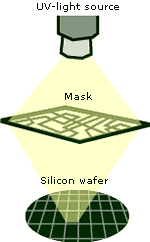
\includegraphics[width=0.35\textwidth]
	{pics/steping.png}
	\caption{Produksi Chip Moderen}
	\label{fig:produksiChipModeren}
\end{figure}

Chip pada zaman sekarang berbasis pada photolithography. Pada teknik ini digunakan radiasi sinar Ultra Violet yang melewati sebuah mask menuju lembaran silikon yang di lapisi filem photosensitive untuk membentuk suatu rangkaian.

\subsection{Kemungkinan Serangan Desain LSI}
Dilihat dari proses developing, terdapat 2 cara untuk mendapatkan sebuah desain untuk di kloning. Pertama dengan mengambil langsung data mentah desain atau "blueprint" dan Reverse Engineering saat barang telah dipublikasi di pasaran.

\begin{figure}
	\centering
	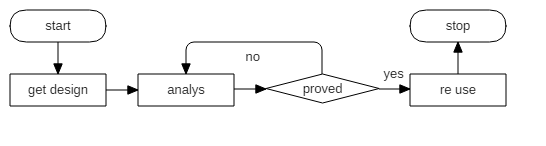
\includegraphics[width=1.05\textwidth]
	{diagrams/untrustSource.png}
	\caption{Clonning/Sumber Tidak Terpercaya}
	\label{fig:untrustsource}
\end{figure}

Dalam segi ini serangan dilakukan dengan cara mencuri langsung desain yang sudah siap di fabrikasi serta uji coba kebenaran. Bila pencuri mendapatkan desain yang telah di uji coba, maka pencuri tinggal langsung memperbanyak desain yang telah di curi.

\begin{figure}
	\centering
	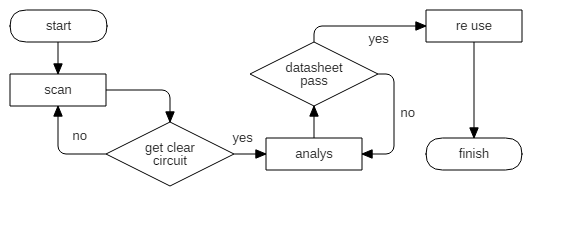
\includegraphics[width=1.05\textwidth]
	{diagrams/reverseEngineering.png}
	\caption{RE (Reverse Engineering)}
	\label{fig:reverseengineering}
\end{figure}

Untuk serangan jenis ini, pencuri sudah pendapatkan produk dari pasar yang telah teruji, pencuri tinggal melakukan scan rangkaian kemudian mengujinya dengan datasheet. Apabila hasil scan desain produk di dapati rangkaian yang konkrit/jelas dan rangkaian tersebut telah teruji sesuai datasheet. Maka pencuri tinggal melakukan fabrikasi.

\subsection{Mengatasi Serangan terhadap Desain LSI}
Dengan meninjau kemungkinan dari tipe serangan, terdapat berbagai cara untuk mengatasi setiap serangan serangan tersebut. Dari reverse engineering hingga untrust source. untuk reverse enginering digunakan teknik anti reverse engineering dan untuk untrust source digunakan teknik identifier dan dengan enclosure agreement law.

\begin{figure}
	\centering
	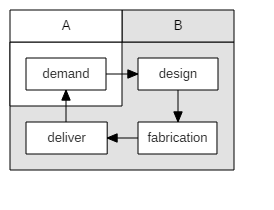
\includegraphics[width=0.5\textwidth]
	{diagrams/oldBusinessLSI.png}
	\caption{Model Bisnis Lama}
	\label{fig:oldbiss}
\end{figure}

Pada model gambar diatas, kegiatan desain, fabrikasi dan deliveri di lakukan oleh satu pihak yang sama. Proses pembuatan suatu perangkat IC dimonopoli oleh 1 perusahaan. Sehingga kemungkinan serangan hanya ada di antara pihak A dan Pihak B.

\begin{figure}
	\centering
	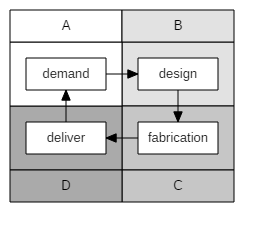
\includegraphics[width=0.5\textwidth]
	{diagrams/newBusinessLSI.png}
	\caption{Model Bisnis Baru}
	\label{fig:newbiss}
\end{figure}

Namun seiring dengan perkembangnya jaman. Monopoli proses dari desain, fabrikasi hingga deliveri mulai sulit di terapkan. Karena dengan semakin berkembangnya jaman dan deman akan fitur desain semakin tinggi, otomatis biaya semakin tinggi dan kompleksitas suatu desain semakin rumit serta waktu untuk menyelesaikan suatu desain semakin lama.

Oleh karena itu sekarang mulai diterapkan Fabless manufakturing atau joint venture untuk membuat suat perangkat elektronika. Setidaknya pada proses bisnis ini terdapat 4 pihak. Pihak A dari keinginan pasar, pihak B yang melakukan perancangan desain, pihak C yang elakukan fabrikasi hasil rancangan pihak B dan Pihak D yang melakukan deliveri hasil fabrikasi di pihak C ke A.

\section{Teknik Proteksi}
Dari berbagai teknik yang telah digunakan, penulis melakukan penggabungan 2 teknik pengamanan dalam sebuah desain IC. Dalam penelitian ini dilakukan penggabungan 2 teknik agar cakupan wilayah keamanan sebuah IC semakin luas. Berikut teknik yang digabungkan dalam penelitian kali ini.

\subsection{Digital Signal Processing Filter}
Digital Signal Prosesing (DSP) merupakan pengolahan sinyal digital, seperti digunakan pada komputer hingga untuk melakukan berbagai operasi proses sinyal. Sinyal yang diproses merupakan kumbulan bilangan sekuensial yang merepresentasikan sampel dari variabel sinyal kontinyu pada suatu domain seperti domain waktu, ruang atau frekuensi.

Pada pengolahan sinyal, sebuah filter adalah sebuah alat atau proses yang menghilangkan beberapa komponen atau fitur yang tidak di inginkan dari suatu sinyal. Filtering merupakan kelas proses sinyal, 

\subsection{Polimorphisme Gate}
Polimorphisme Gate merupakan teknik pengecoh yang di gunakan dalam perlindungan desain IC. Sebagai contoh sebuah rangkaian dengan ouput F dan input A,B dan C akan memiliki hasil yang berbeda jika parameters k yang diberikan berbeda. Misal bila parameter k diisi dengan kombinasi 0101 maka outputnya adalah
\begin{center}
	F = A XOR (A \textbf{AND} B)
\end{center}
Sedangkan bila parameter k diisi dengan kombinasi 1101 maka outputnya menjadi
\begin{center}
	F = A XOR (A \textbf{NOR} B)
\end{center}

\begin{figure}
	\centering
	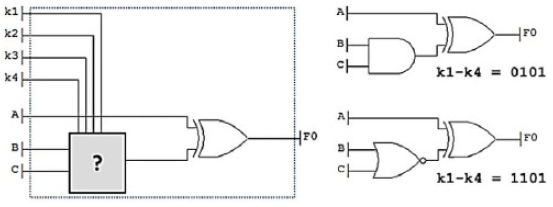
\includegraphics[width=0.75\textwidth]
	{pics/polymorphgate.png}
	\caption{Polymorph gate}
	\label{fig:poly}
\end{figure}

\section{Peralatan dan Teknologi}
Dalam penelitian kali ini dibutuhkan beberapa peralatan dan standard teknologi untuk mengembangkan teknik perlindungan intelektual properti. Sebagai penunjang dalam pembuatan perlindungan, penulis menggunakan tools dan teknologi yang umum digunakan dalam proses pengembangan desain LSI.

\subsection{Verilog HDL}
Verilog HDL merupakan bahasa pendeskripsi hardware yang digunakan untuk mendesain dan dokumentasi sistem elektronika. Verilog HDL memungkinkan perancang mendesain pada berbagai tingkatan abstraksi.

Verilog HDL berasal dari Automated Integrated Design System (yang kemudian berubah nama menjadi Gateway Design Automation) pada tahun 1985. Saat itu perusahaan tersebut dipegang oleh Dr. Prabhu Goel, pendiri PODEM test generation algorithm. Verilog HDL di desain oleh Phil Moorby, yang kemudian menjadi chief Designer untuk Verilog-XL dan perusahaan rekan pertama di Cadance Design System. 

Awalnya Verilog dibuat sebagai bahasa simulasi. Kemudian setelah berkembang tidak hanya digunakan untuk simulasi namun juga untuk sintesis. (source www.verilog.com)

\subsection{Python}
Python merupakan High-Level Programming Language yang banyak digunakan untuk general purpose programming, di buat oleh Guido van Rossum dan pertamakali rilis pada tahun 1991. Sebuah pahasa Interpretasi, Python memiliki filosofi disain yang meng emphasis code readibility, dan sintax yang memungkinkan programmer mengekspresikan konsep pada beberapa line of code dari pada yang digunakan pada bahasa lain seperti C++ atau Java. (source Kuhlman, Dave. "A Python Book: Beginning Python, Advanced Python, and Python Exercises"... Summerfield, Mark. Rapid GUI Programming with Python and Qt. Python is a very expressive language, which means that we can usually write far fewer lines of Python code than would be required for an equivalent application written in, say, C++ or Java)

Python memiliki fitur sistem tipe dinamis dan memori manajemen otomatis serta mendukung multiple paradigma programming, termasuk Objek-orientasi, Imperative, Functional program, dan prosedural style. Bahasa ini juga memiliki banyak librari standard yang komperhensif. (source "About Python". Python Software Foundation. Retrieved 24 April 2012., second section "Fans of Python use the phrase "batteries included" to describe the standard library, which covers everything from asynchronous processing to zip files.")

Python interpraters tersedia pada berbagai macam platform sistem operasi, memungkinkan kode Python berjalan pada berbagai macam sistem. (source "History and License". Retrieved 5 December 2016. "All Python releases are Open Source")

\subsection{Yosys Open SYnthesis Suite}
Yosys adalah sebuah framework untuk sintesis Verilog RTL. Sekarang ini memiliki suport yang extensif pada Verilog-2005 dan mendukun berbagai set basik algoritma sintesis untuk berbagai domain aplikasi.

\begin{figure}
	\centering
	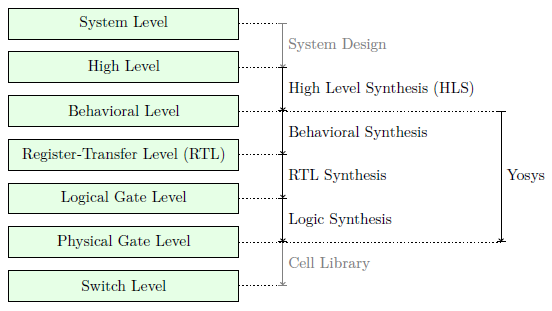
\includegraphics[width=0.75\textwidth]
	{pics/yosys.png}
	\caption{Perbedaan Tinkatan Abstraksi dan Sintesis Yosys}
	\label{yosys}
\end{figure}

\subsection{Liberty Timing File (.lib)}
Liberty adalah

\subsection{Electric's native file format (.jelib)}
Liberty adalah

\subsection{Graphic Database System (.gds)}
Graphic Data System merupakan format file database yang menyimpan informasi grafis. Format file ini sering digunakan sebagai penyimpanan layout IC yang siap di fabrikasi.

\subsection{Electric VLSI}

\begin{figure}
	\centering
	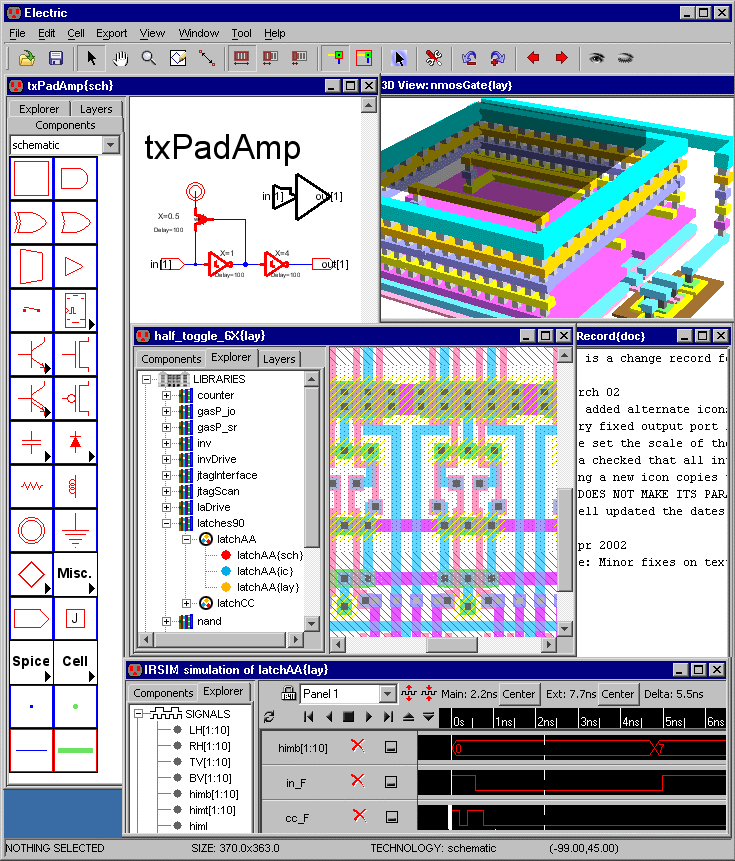
\includegraphics[width=0.75\textwidth]
	{pics/electricvlsi.png}
	\caption{Tampilan Electric VLSI}
	\label{fig:vlsi}
\end{figure}

\subsection{Xilinx ISE Design Suit}
Xilinx ISE Design Suit merupakan Computer Aided Design (CAD) keluaran Xilinx yang digunakan untuk developing IC.

\begin{figure}
	\centering
	
\includegraphics[width=0.4\textwidth]
	{pics/ise-logo.jpg}
	\caption{Logo Xilinx ISE Design Suit}
	\label{ise}
\end{figure}

\subsection{FPGA Elbert V2 Board}
FPGA merupakan kepanjangan dari Field Programmable Gate Array adalah perangkat keras yang biasa digunakan dalam proses manufakturing IC. FPGA digunakan untuk mensimulasikan draft rancangan IC yang siap untuk di test yang apabila telah lolos test akan di lanjutkan ke tahap layout. FPGA hanya digunakan apabila rancangan membutuhkan input dari perangkat lain atau program kernel.

\begin{figure}
	\centering
	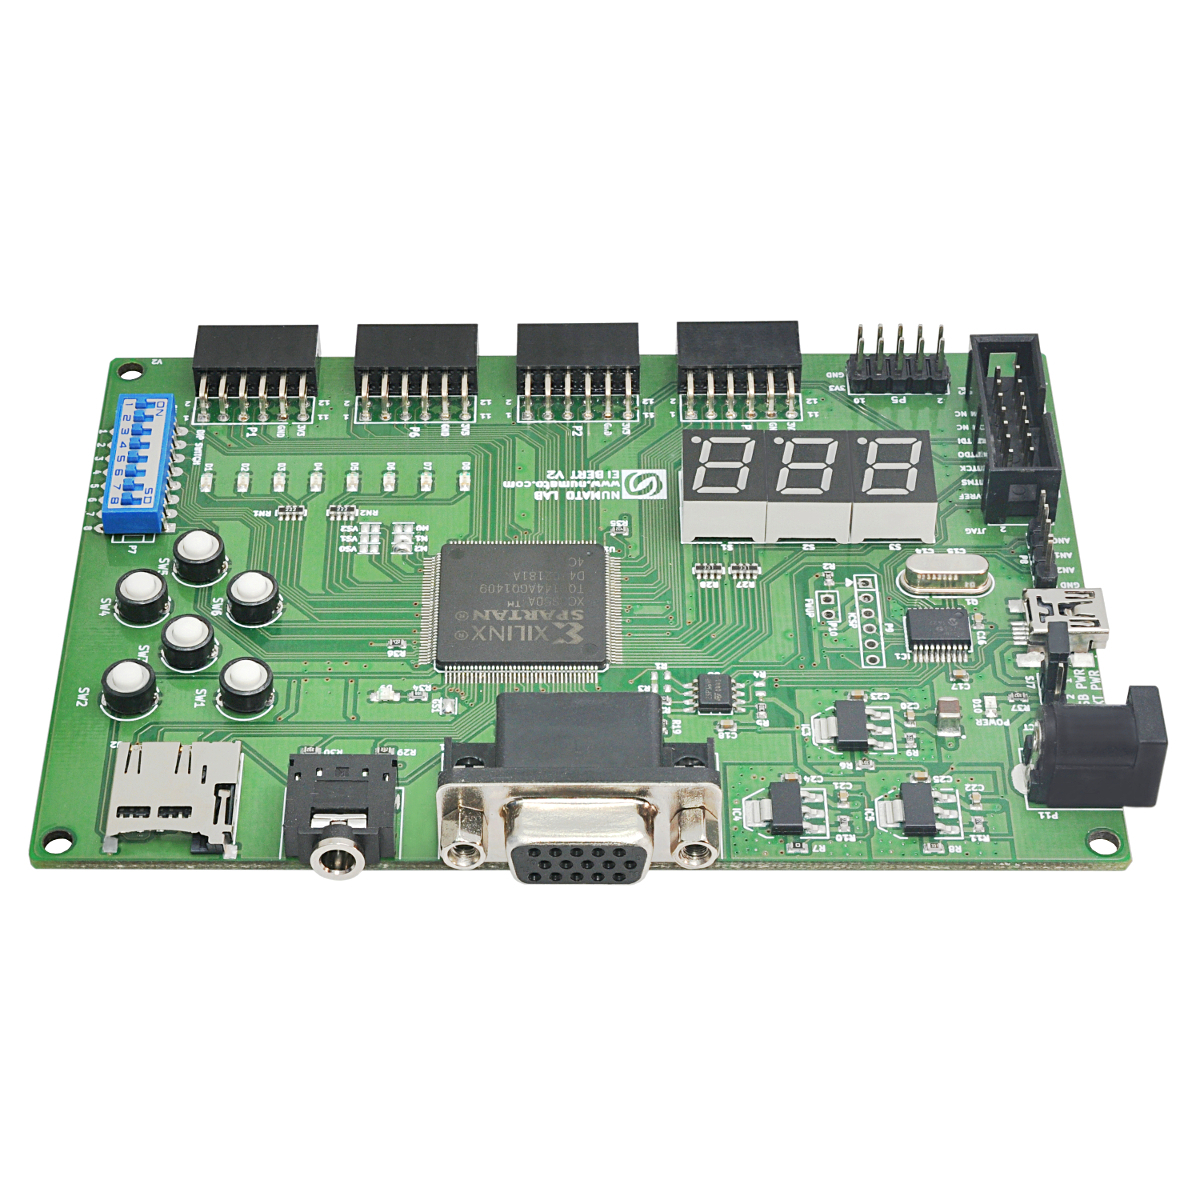
\includegraphics[width=0.75\textwidth]
	{pics/elbertv2.jpg}
	\caption{FPGA Board - Elbert V2}
	\label{fig:fpga}
\end{figure}

Elbert V2 merupakan Board yang simple namun serbaguna untuk pembelajaran atau pengembangan. Board ini menggunakan Xilinx Spartan 3A FPGA. Pada Development Board ini memiliki fitur FPGA dari Xilinx XC3S50A dengan 144 pin dengan maksimum 108 user IO. Dilengkapi dengan antarmuka USB2 untuk kemudahan konfigurasi ke SPI flash. 

\subsection{Mikrokontroler}
Mikrokontroler adalah sebuah perangkat chip elktronika yang berfungsi sebagai kontroler. Di dalam perangkat mikrokontroler setidaknya terdapat ALU, Memory, IO.

\section{Target IP Core}
Watermark adalah rangkaian yang tidak boleh berdiri sendiri pada implementasinya walaupun dalam pengembangannya bisa di lakukan mandiri. Dalam penelitian kali ini Module yang akan di watermark adalah modul ALU.

\subsection{Aritmatic Logic Unit (ALU)}
Aritmatik Logic Unit (ALU) adalah kombinasi rangkaian elektronik digital yang melakukan fungsi aritmatika dan operasi bitwise pada bilangan integer binari. Ini sangat kontras dengan Floating Point Unit (FPU), yang melakukan operasi bilangan floating point. Sebuah ALU pada dasarnya bagian dari berbagai macam blok rangkaian komputasi, termasuk Central Prosesing Unit (CPU). Sebuah CPU, FPU, atau GPU mungkin memiliki banyak ALU di dalamnya.

\begin{figure}
	\centering
	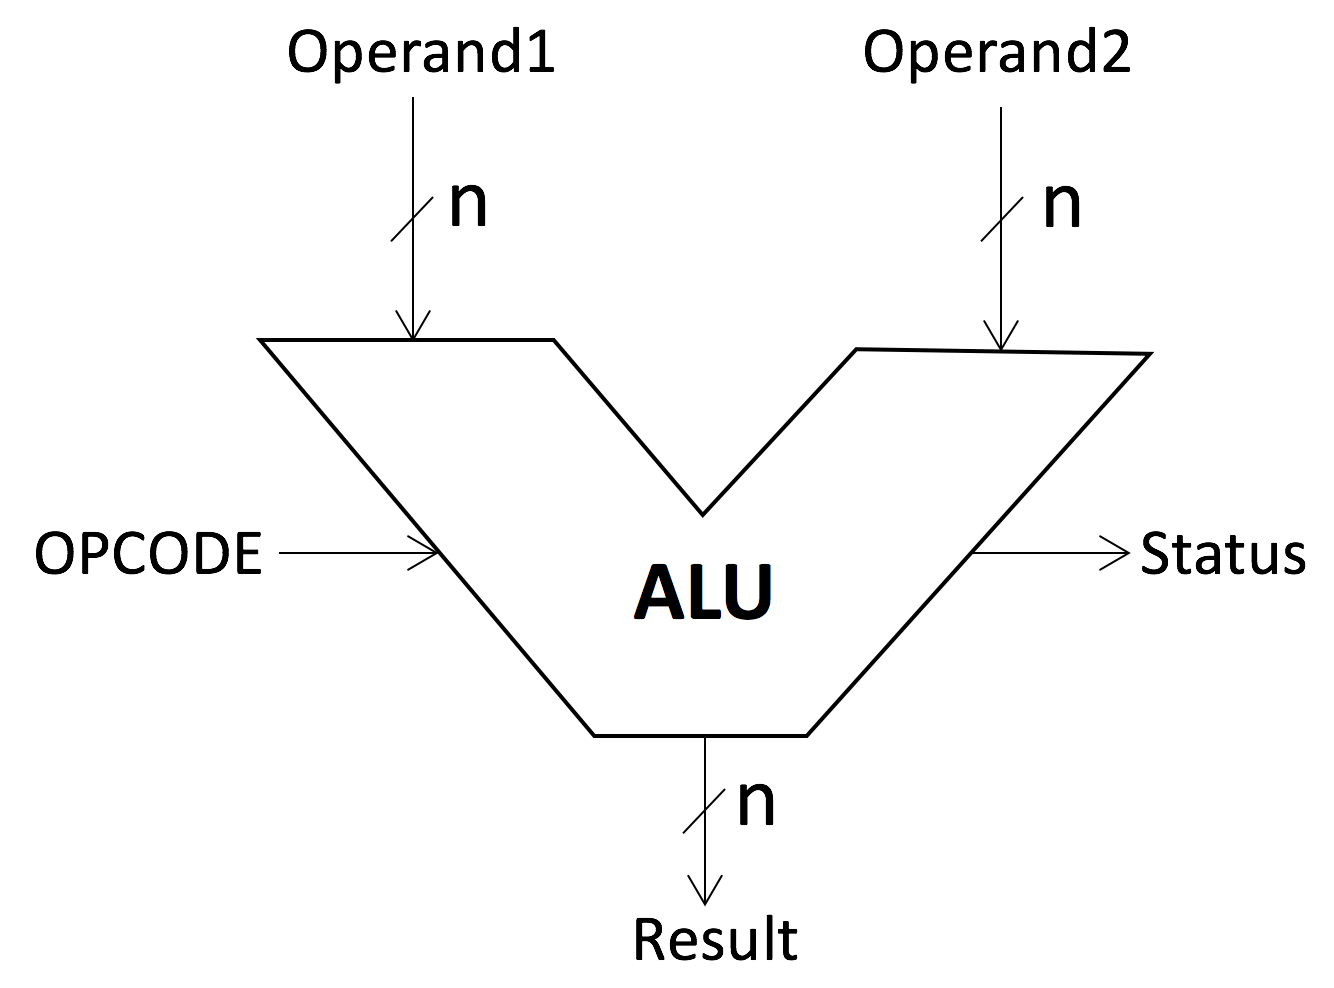
\includegraphics[width=0.5\textwidth]
	{pics/alu.png}
	\caption{ALU}
	\label{alu}
\end{figure}


%%%%%%%%%%%%%%%%%%%%%%%%%%%%%%%%%%%%%%%%%%%%%%%%%%%%%%%%%%%%%%%%%%%%%%%
% 
%%%%%%%%%%%%%%%%%%%%%%%%%%%%%%%%%%%%%%%%%%%%%%%%%%%%%%%%%%%%%%%%%%%%%%%

\chapter{\babTiga}
Perancangan serta langkah-langkah di perlukan untuk menyelesaikan penelitian ini. Berikut ini akan di jelaskan gambaran serta tahapan dari perancangan system yang di teliti serta skenario simulasi dari hasil desain yang telah dirancang.

%%%%%%%%%%%%%%%%%%%%%%%%%%%%%%%%%%%%%%%%%%%%%%%%%%%%%%%%%%%%%%%%%%%%%%%
% 
%%%%%%%%%%%%%%%%%%%%%%%%%%%%%%%%%%%%%%%%%%%%%%%%%%%%%%%%%%%%%%%%%%%%%%%

\section{Perancangan Desain}

Desain utama adalah desain modul alu. Pada penelitian kali ini digunakan modul ALU dengan 2 register masing-masing 8 bit input, 4 bit opcode dan 8 bit output seperti ditunjukan pada diagram dibawah ini.

\begin{figure}
	\centering
	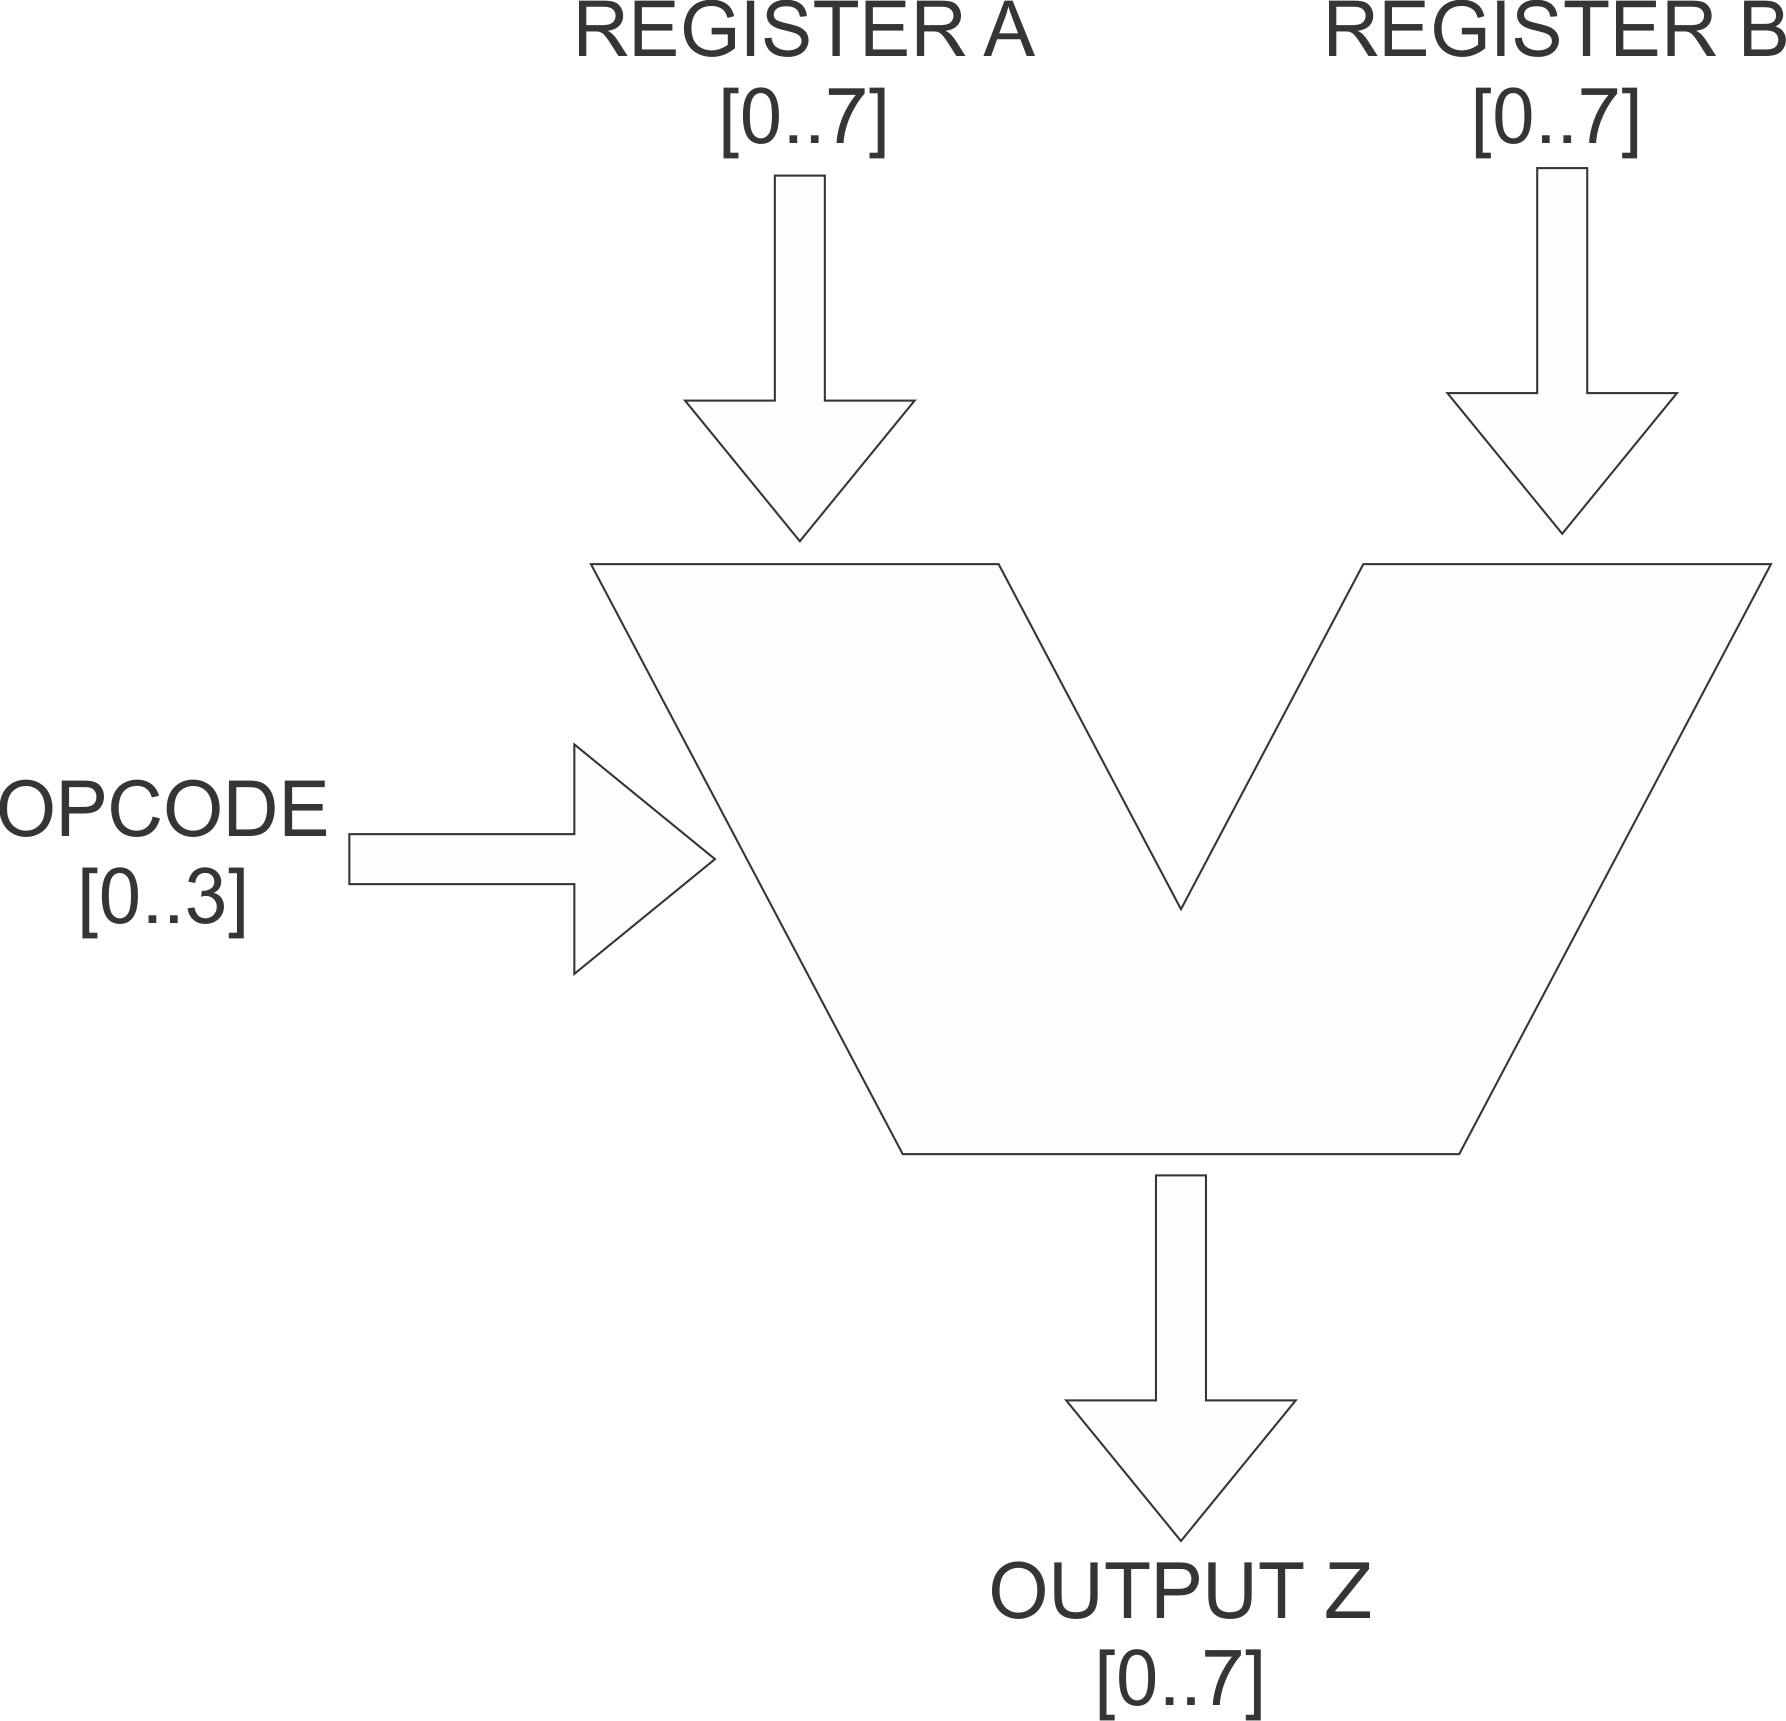
\includegraphics[width=0.5\textwidth]
	{ilustrasi/aludesain.png}
	\caption{Desain ALU yang akan dilindungi}
	\label{aludesain}
\end{figure}

Selain menggunakan desain ALU penulis juga merancang desain perlindungan dengan input 4 bit dan output 8 bit seperti yang ditunjukan diagram dibawah ini. modul inilah yang nantinya akan diselipkan pada modul ALU.

\begin{figure}
	\centering
	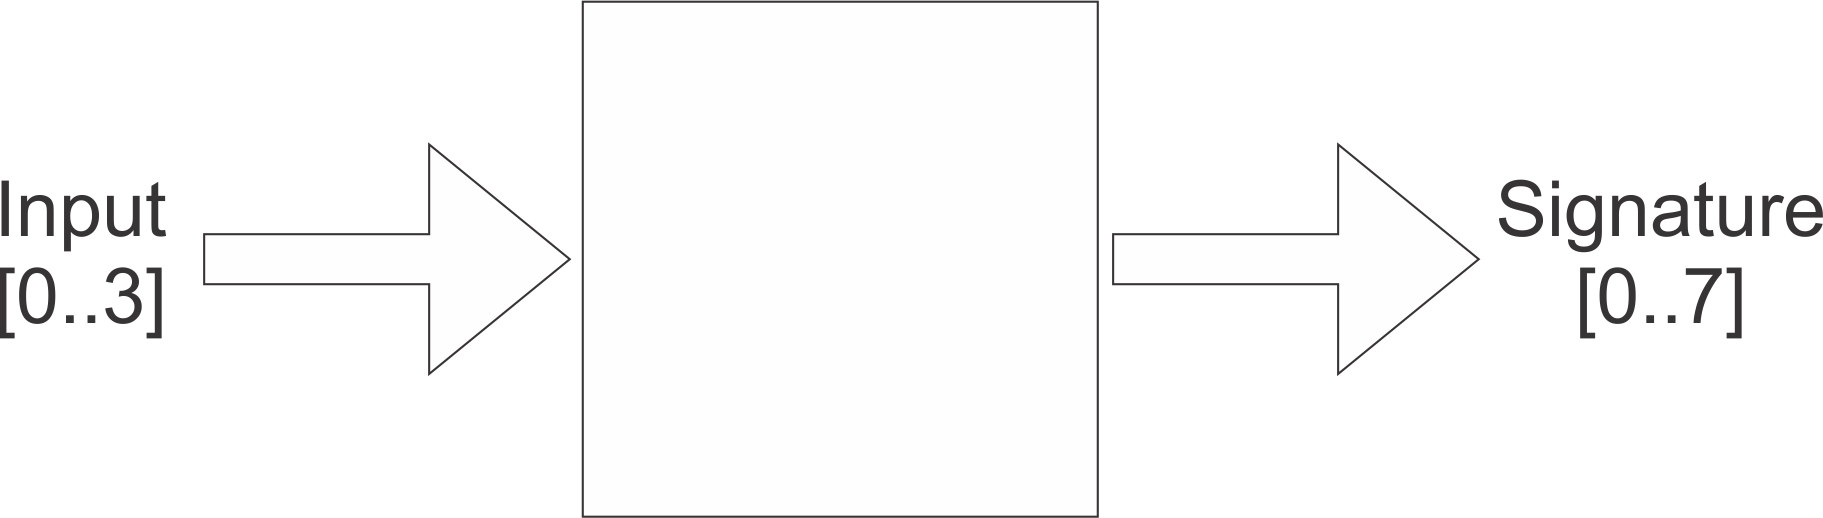
\includegraphics[width=0.5\textwidth]
	{ilustrasi/watermarkdesain.png}
	\caption{Desain rangkaian pelindung}
	\label{watermarkdesain}
\end{figure}

\subsection{Skema Perlindungan}

Skema perlindungan ini dilakukan teknik Pengolahan Sinyal Digital untuk ekstraksi data signature dan obfuscation dengan polymorph gate untuk menyembunyikan keberadaan signature. Dibawah berikut merupakan spesifikasi I/O pada modul yang akan dilindngi.

\begin{figure}
	\centering
	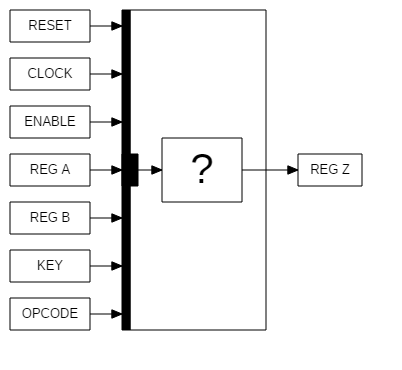
\includegraphics[width=0.5\textwidth]
	{diagrams/topAsk.png}
	\caption{Desain rangkaian Top modul yang terdapat rangkaian lain}
	\label{topAsk}
\end{figure}

Untuk teknik obfuscation dengan polymorph dilakukan desain yang bertujuan menyelipkan suatu modul lain pada modul utama tanpa diketahui pengguna. Teknik ini seperti memberikan program Trojan kedalam suatu program utama. Namun sub-program ini bukan untuk merusak namun untuk melindungi. Seperti ilustrasi di atas menunjukan suatu modul besar namun ada sesuatu lain di dalam modul tersebut.

\begin{figure}
	\centering
	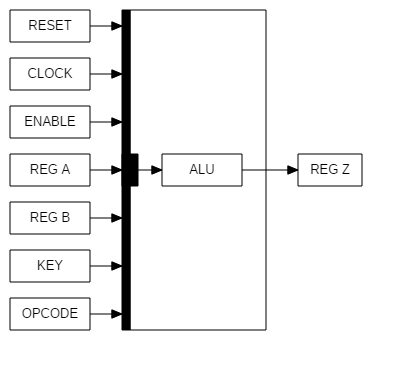
\includegraphics[width=0.5\textwidth]
	{diagrams/topAlu.png}
	\caption{Desain rangkaian ALU pada top modul}
	\label{topAlu}
\end{figure}

Pertama penulis menggunakan rangkaian ALU sebagai modul besar (utama) dengan spesifikasi I/O chip yang telah ditentukan sebelumnya. Lalu fungsional ALU ditest dengan spesifikasi yang telah dibuat. 

\begin{figure}
	\centering
	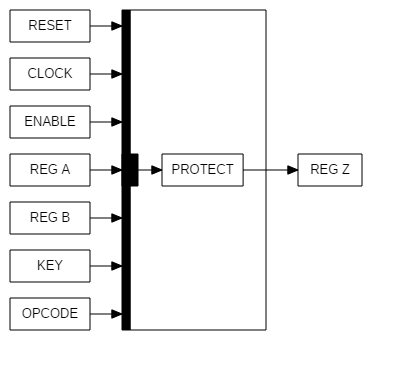
\includegraphics[width=0.5\textwidth]
	{diagrams/topPro.png}
	\caption{Desain rangkaian pelindung pada top modul}
	\label{topPro}
\end{figure}

Setelah itu ganti rangkaian modul ALU dengan modul perlindungan sebagai modul utama kemudian dilakukan tes fungsional kembali untuk mengetahui apakah rangkaian perlindungan dapat bekerja diatas arsitektur serta spesifikasi modul utama.

Setelah didapat kedua modul dapat berjalan sesuai dengan semestinya maka langkah selanjutnya menggabungkan kedua modul tersebut bada modul utama. pada penggabungan kali ini digunakan teknik obfucation polymorph untuk memilih antara modul mana yang harus berjalan pada modul utama.

\begin{figure}
	\centering
	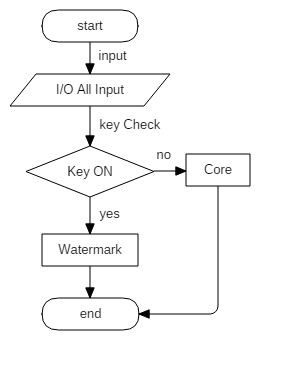
\includegraphics[width=0.5\textwidth]
	{diagrams/Activation.png}
	\caption{Algoritma aktifasi}
	\label{fig:aktifasi}
\end{figure}

Diagram diatas menunjukan bagaimana cara mengaktifkan modul dengan key sebagai kontroler. Untuk hasil outpu diperlukan kontrol tambahan penjembatan antara hasil output modul ALU dan modul perlindungan seperti pada ilustrasi di bawah agar tidak terjadi bentrokan antara kedua output,

\begin{figure}
	\centering
	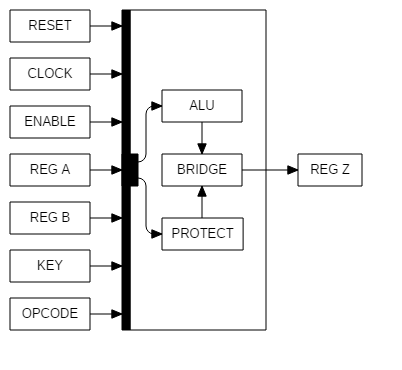
\includegraphics[width=0.5\textwidth]
	{diagrams/top.png}
	\caption{Desain rangkaian top modul yang telah diberi pelindung}
	\label{top}
\end{figure}

dibawah ini merupakan contoh listing program pada ilustrasi di atas. Sehingga terdapat 1 Top modul dan 3 sub modul pada desain chip yang telah diberikan rangkaian pelindung.\\\\

\begin{lstlisting}[language=Verilog, caption=Listing Top Modul]
// Main Modul IC Watermark
module alu( RST, CLK, ENA, RGA, RGB, RGZ, KEY, OPT);
    // Deklarasi I/O
    input  RST, CLK, ENA;
    input  [3:0]OPT;
    input  [7:0]RGA,RGB;
    input  [1:0]KEY;
    output [7:0]RGZ;
    wire   [7:0]A,B,RGZ;
    // Core Inti
    alu_min aluj(RST, CLK, ENA, RGA, RGB, A, KEY, OPT);
    // Protektor
    protection prot(RST, CLK, ENA, RGA, RGB, B, KEY);
    // Bridge antara core dan protektor
    bridge jembatan(A, B, RGZ);
endmodule
\end{lstlisting}

\subsection{Spesifikasi}
Spesifikasi rangkaian dapat dilihat di lampiran.

%%%%%%%%%%%%%%%%%%%%%%%%%%%%%%%%%%%%%%%%%%%%%%%%%%%%%%%%%%%%%%%%%%%%%%%
% 
%%%%%%%%%%%%%%%%%%%%%%%%%%%%%%%%%%%%%%%%%%%%%%%%%%%%%%%%%%%%%%%%%%%%%%%

\section{Alur Proses Pengembangan}
Secara garis besar pada sisi desainer, terdapat 3 langkah untuk melakukan pengembangan alat dari programming hingga layout siap cetak. Penulis menggunakan cara ini dari hasil studi serta eksperimen saat proses pengembangan alat.

\begin{figure}
	\centering
	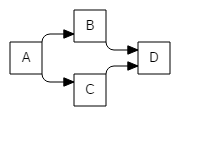
\includegraphics[width=0.3\textwidth]{diagrams/All_General.png}
	\caption{Skema Perancangan Umum Proses Desain}
\end{figure}

Pada langkah pertama dilakukan proses A, penulis melakukan perancangan desain dari IC yang akan di watermark kemudian di lakukan analisis. Apabila pertama telah selesai, penulis akan melakukan langkah kedua. Pada langkah kedua ini di lakukan kegiatan B yaitu proses ferifikasi dengan FPGA dan kegiatan C yaitu proses syntesys menjadi Raw Layout. Setelah kegiatan B dan C selesai maka kegiatan D yaitu proses finalisasi layout dapat dilakukan yang akhirnya hasil final layout dapat di serahkan ke pabrik untuk di fabrikasi.

\begin{figure}
	\centering
	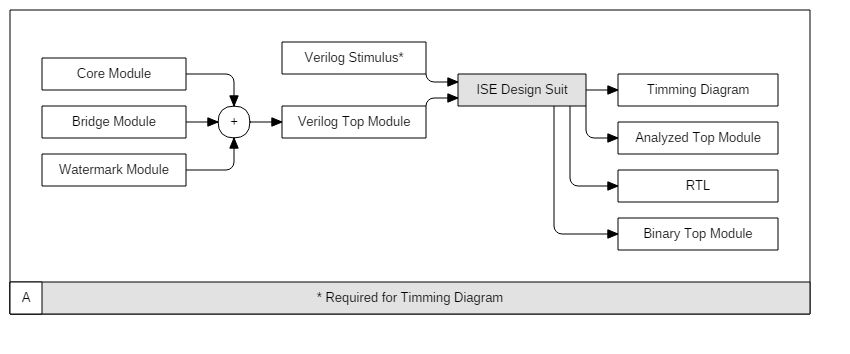
\includegraphics[width=1.0\textwidth]
	{diagrams/kegiatanA.png}
	\caption{Skema kegiatan A}
	\label{kegiatanA}
\end{figure}

Secara umum pada kegiatan A, penulis membuat 3 module verilog untuk digabungkan. Core Module yaitu program rangkaian ALU, Watermark Module adalah program untuk watermarking dan Bridge Module untuk menghubungkan output antara Core Module dan Watermark Module. Setelah selesai dilakukan programming setiap medule tersebut maka medul-modul tadi digabungkan menjadi Top Module. Top Module ini lah yang nantinya akan menjadi IC terwatermark. 

Pada top module ini harus diberikan program tambahan yaitu stimulus untuk dapat mensimulasikan skenario Input dan Output dari Top Module. Bila sekenario stimulus telah dibuat, kemudian dilakukan simulasi dengan bantuan softwere ISE design suit untuk melihat hasil simulasi berupa Timming diagram. Pada Timming Diagram inilah dapat di lihat apakah sekenario dari Input dan Output sesuai dengan keinginan. Setelah hasil analisis sesuai dengan yang diinginkan maka dilanjutkan dengan kegiatan selanjutnya yaitu kegiatan B dan C.

\begin{figure}
	\centering
	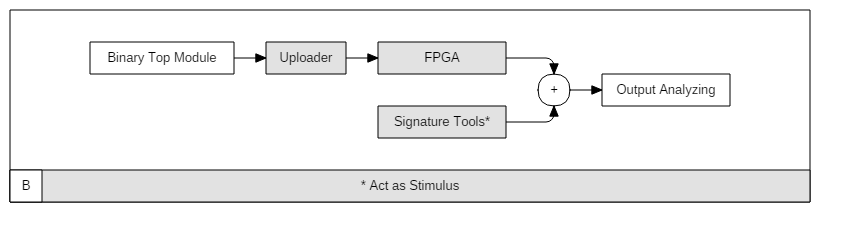
\includegraphics[width=1.0\textwidth]
	{diagrams/kegiatanB.png}
	\caption{Skema kegiatan B}
	\label{kegiatanB}
\end{figure}

Pada kegiatan B ini dilakukan simulasi ferivikasi pada board FPGA dengan alat ferifikasi. kegiatan ini dilakukan untuk simulasi ferifikasi signature pada IC yang telah diwatermark. IC yang telah diwatermak di tanam pada FPGA dan dengan menggunakan Signature Tools dilakukan ferifikasi sehingga didapat data signature dari IC yang telah di watermask.

\begin{figure}
	\centering
	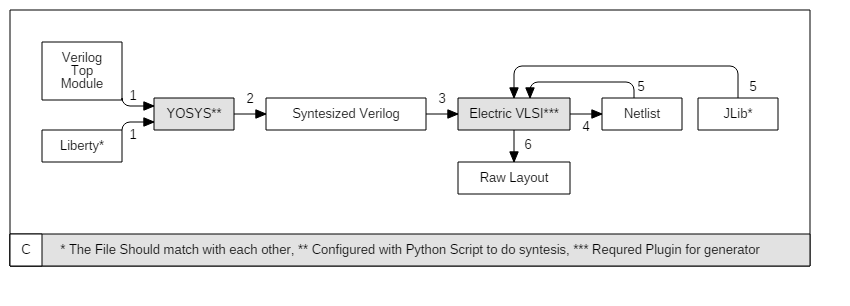
\includegraphics[width=1.0\textwidth]
	{diagrams/kegiatanC.png}
	\caption{Skema kegiatan C}
	\label{kegiatanC}
\end{figure}

Untuk kegiatan C dilakukan developing layout dari Top Module yang telah diferifikasi dengan timming diagram. Defeloping menggunakan softwere Electric VLSI. Dengan mensyntesis Verilog Top Module dan Liberty file menggunakan YOSYS, maka akan di dapat file verilog tersyntesis. Kemudian File tersintesis tersebut di Load di Electric VLSI untuk di rubah ke NetList. Setelah berhasil di rubah menjadi NetList maka file NetList tersebut di kompilasi bersama file JLib pada electric VLSI untuk di jadikan Raw Layout.

\begin{figure}
	\centering
	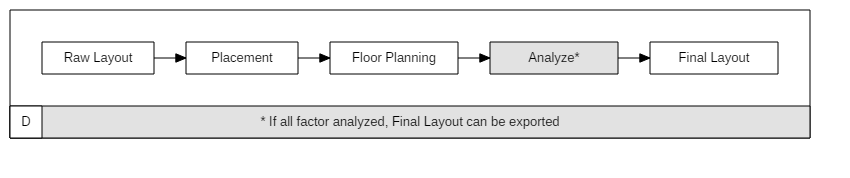
\includegraphics[width=1.0\textwidth]
	{diagrams/kegiatanD.png}
	\caption{Skema kegiatan D}
	\label{kegiatanD}
\end{figure}

Pada tahap ini di lakukan kegiatan C yaitu memproses Raw Layout menjadi Final Layout yang siap di cetak. Tahapan nya adalah melakukan placement untuk setiap modulnya lalu di lakukan analisis kemudian dilakukan Floor planning. Setelah itu dilakukan analisis kembali hingga didapat hasil yang terbaik. Apabila telah didapat hasil yang terbaik maka File siap untuk difabrikasi.

%%%%%%%%%%%%%%%%%%%%%%%%%%%%%%%%%%%%%%%%%%%%%%%%%%%%%%%%%%%%%%%%%%%%%%%
% 
%%%%%%%%%%%%%%%%%%%%%%%%%%%%%%%%%%%%%%%%%%%%%%%%%%%%%%%%%%%%%%%%%%%%%%%

\section{Simulasi}
Simulasi dilakukan pada 2 environment, yaitu simulasi softwere (Timming diagram) serta simulasi hardwere (FPGA). Simulasi Timming diagram menggunakan simulator multisim yang tersedia sebagai fitur dari ISE Design Suit. Fitur ini bisa digunakan dengan langsung menjalankan simulator pada Top modul dan memasukan sinyal yang akan ditest atau menggunakan kode tambahan sebagai testbench. Keuntungan menggunakan tesbench ini kita bisa mengatur skenario simulasi pada top modul dan mempermudah dalam melakukan uji perangkat bila banyak sinyal dan faktor yang perlu di uji.

\begin{figure}
	\centering
	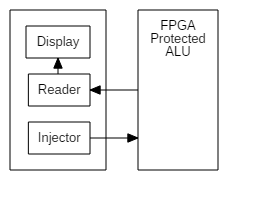
\includegraphics[width=0.5\textwidth]
	{diagrams/SimulasiAlat.png}
	\caption{Simulasi Alat}
	\label{SimulasiAlat}
\end{figure}

\chapter{\babEmpat}
\todo{tambahkan kata-kata pengantar bab 4 disini}

\section{Pengujian}
\todo{Tampilkan macam macam hasil pengujian yang telah di lakukan}

\subsection{Sekenario Pengujian}
\todo{tambahin kata kata}

\subsection{Hasil Pengujian}
\todo{tambahin kata kata}

\section{Analisis}
\todo{Tampilkan macam macam hasil analisis dari setiap pengujian}

\chapter{\babLima}
\todo{Tambahkan kata-kata pengantar bab 5 disini.}

\section{Mengubah Tampilan Teks}

Beberapa perintah yang dapat digunakan untuk mengubah tampilan adalah: 
\begin{itemize}
	\item \bslash f \\
		Merupakan alias untuk perintah \bslash textit, contoh 
		\f{contoh hasil tulisan}.
	\item \bslash bi \\
		\bi{Contoh hasil tulisan}.
	\item \bslash bo \\
		\bo{Contoh hasil tulisan}.
	\item \bslash m \\
		\m{Contoh hasil tulisan}.
	\item \bslash mc \\
		\mc{Contoh hasil tulisan}.
	\item \bslash code \\ 
		\code{Contoh hasil tulisan}.
\end{itemize}

\section{Memberikan Catatan}

Ada dua perintah untuk memberikan catatan penulisan dalam dokumen yang Anda kerjakan, yaitu: 
\begin{itemize}
	\item \bslash todo \\
		Contoh: \\ \todo{Contoh bentuk todo.}
	\item \bslash todoCite \\ 
		Contoh: \todoCite
\end{itemize}

\section{Menambah Isi Daftar Isi}

Terkadang ada kebutuhan untuk memasukan kata-kata tertentu kedalam Daftar Isi. Perintah \bslash addChapter dapat digunakan untuk judul bab dalam Daftar isi. Contohnya dapat dilihat pada berkas thesis.tex.

\section{Memasukan PDF}

Untuk memasukan PDF dapat menggunakan perintah \bslash inpdf yang menerima satu buah argumen. Argumen ini berisi nama berkas yang akan digabungkan dalam laporan. PDF yang dimasukan degnan cara ini akan memiliki header dan footer seperti pada halaman lainnya. 

\inpdf{include}

Cara lain untuk memasukan PDF adalah dengan menggunakan perintah \bslash putpdf dengan satu argumen yang berisi nama berkas pdf. Berbeda dengan perintah sebelumnya, PDF yang dimasukan dengan cara ini tidak akan memiliki footer atau header seperti pada halaman lainnya. 

\putpdf{include}

\section{Membuat Perintah Baru}

Ada dua perintah yang dapat digunakan untuk membuat perintah baru, yaitu: 
\begin{itemize}
	\item \bslash Var \\
		Digunakan untuk membuat perintah baru, namun setiap kata yang diberikan akan diproses dahulu menjadi huruf kapital. Contoh jika perintahnya adalah \bslash Var\{adalah\} makan ketika perintah \bslash Var dipanggil, yang akan muncul adalah ADALAH. 
	\item \bslash var \\
		Digunakan untuk membuat perintah atau baru. 
\end{itemize}
\chapter{\babEnam}
\todo{tambahkan kata-kata pengantar bab 6 disini}


\chapter{\kesimpulan}
\todo{Tambahkan kesimpulan dan saran terkait dengan perkerjaan 
	yang dilakukan.}

\section{Kesimpulan}

\section{Saran}



% Daftar Pustaka
\begin{thebibliography}{4}

\bibitem{latex.intro}
{Jeff Clark. (n.d). \f{Introduction to LaTeX}. 26 Januari 2010. \url{http://frodo.elon.edu/tutorial/tutorial/node3.html}.}

\end{thebibliography}



% Lampiran 
\begin{appendix}
	\begin{titlepage}
	\centering 
	\vspace*{6cm}
	\noindent \Huge{LAMPIRAN}
	\addChapter{LAMPIRAN}
\end{titlepage}
	\setcounter{page}{2}
	\addChapter{Lampiran 1}
\chapter*{Lampiran 1}

% Table generated by Excel2LaTeX from sheet 'Mechines'
\begin{table}[htbp]
	\centering
	\caption{Add caption}
	\begin{tabular}{|c|r|r|r|}
		\hline
		\rowcolor[rgb]{ .851,  .851,  .851} \multicolumn{4}{|c|}{Keterangan Type} \bigstrut\\
		\hline
		\rowcolor[rgb]{ .851,  .851,  .851} n & \multicolumn{1}{c|}{\cellcolor[rgb]{ 1,  1,  1}LITER} & \multicolumn{2}{c|}{\cellcolor[rgb]{ 1,  1,  1}METER} \bigstrut\\
		\hline
		\rowcolor[rgb]{ .851,  .851,  .851} \textbf{A} & \cellcolor[rgb]{ 1,  1,  1}10 & \cellcolor[rgb]{ 1,  1,  1}0,01 & \cellcolor[rgb]{ 1,  1,  1}0,0215 \bigstrut\\
		\hline
		\rowcolor[rgb]{ .851,  .851,  .851} \textbf{B} & \cellcolor[rgb]{ 1,  1,  1}100 & \cellcolor[rgb]{ 1,  1,  1}0,1 & \cellcolor[rgb]{ 1,  1,  1}0,0464 \bigstrut\\
		\hline
		\rowcolor[rgb]{ .851,  .851,  .851} \textbf{C} & \cellcolor[rgb]{ 1,  1,  1}1.000 & \cellcolor[rgb]{ 1,  1,  1}1 & \cellcolor[rgb]{ 1,  1,  1}0,1000 \bigstrut\\
		\hline
		\rowcolor[rgb]{ .851,  .851,  .851} \textbf{D} & \cellcolor[rgb]{ 1,  1,  1}10.000 & \cellcolor[rgb]{ 1,  1,  1}10 & \cellcolor[rgb]{ 1,  1,  1}0,2154 \bigstrut\\
		\hline
		\rowcolor[rgb]{ .851,  .851,  .851} \textbf{E} & \cellcolor[rgb]{ 1,  1,  1}100.000 & \cellcolor[rgb]{ 1,  1,  1}100 & \cellcolor[rgb]{ 1,  1,  1}0,4642 \bigstrut\\
		\hline
		\rowcolor[rgb]{ .851,  .851,  .851} \textbf{F} & \cellcolor[rgb]{ 1,  1,  1}1.000.000 & \cellcolor[rgb]{ 1,  1,  1}1K & \cellcolor[rgb]{ 1,  1,  1}1,0000 \bigstrut\\
		\hline
		\rowcolor[rgb]{ .851,  .851,  .851} \textbf{G} & \cellcolor[rgb]{ 1,  1,  1}10.000.000 & \cellcolor[rgb]{ 1,  1,  1}10K & \cellcolor[rgb]{ 1,  1,  1}2,1544 \bigstrut\\
		\hline
		\rowcolor[rgb]{ .851,  .851,  .851} \textbf{H} & \cellcolor[rgb]{ 1,  1,  1}100.000.000 & \cellcolor[rgb]{ 1,  1,  1}100K & \cellcolor[rgb]{ 1,  1,  1}4,6416 \bigstrut\\
		\hline
		\rowcolor[rgb]{ .851,  .851,  .851} \textbf{I} & \cellcolor[rgb]{ 1,  1,  1}1.000.000.000 & \cellcolor[rgb]{ 1,  1,  1}1M & \cellcolor[rgb]{ 1,  1,  1}10,0000 \bigstrut\\
		\hline
		\rowcolor[rgb]{ .851,  .851,  .851} \textbf{J} & \cellcolor[rgb]{ 1,  1,  1}10.000.000.000 & \cellcolor[rgb]{ 1,  1,  1}10M & \cellcolor[rgb]{ 1,  1,  1}21,5443 \bigstrut\\
		\hline
		\rowcolor[rgb]{ .851,  .851,  .851} \textbf{K} & \cellcolor[rgb]{ 1,  1,  1}100.000.000.000 & \cellcolor[rgb]{ 1,  1,  1}100M & \cellcolor[rgb]{ 1,  1,  1}46,4159 \bigstrut\\
		\hline
		\rowcolor[rgb]{ .851,  .851,  .851} \textbf{L} & \cellcolor[rgb]{ 1,  1,  1}1.000.000.000.000 & \cellcolor[rgb]{ 1,  1,  1}1B & \cellcolor[rgb]{ 1,  1,  1}100,0000 \bigstrut\\
		\hline
		\rowcolor[rgb]{ .851,  .851,  .851} \textbf{M} & \cellcolor[rgb]{ 1,  1,  1}10.000.000.000.000 & \cellcolor[rgb]{ 1,  1,  1}10B & \cellcolor[rgb]{ 1,  1,  1}215,4435 \bigstrut\\
		\hline
		\rowcolor[rgb]{ .851,  .851,  .851} \textbf{N} & \cellcolor[rgb]{ 1,  1,  1}100.000.000.000.000 & \cellcolor[rgb]{ 1,  1,  1}100B & \cellcolor[rgb]{ 1,  1,  1}464,1589 \bigstrut\\
		\hline
	\end{tabular}%
	\label{tab:addlabel}%
\end{table}%

\end{appendix}

\end{document}